% !TEX root = ../thesis-example.tex
\chapter{Concepts}
\label{sec:concepts}

In this chapter different ways to evaluate \gls{tessla} specifications are given and their equivalence is shown.
To do so in Section~\ref{sec:concepts:defs} building blocks for evaluation approaches are defined, which are then used in later sections to define behaviour of them and show their equivalence.

\section{Definitions}
\label{sec:concepts:defs}

While the \gls{tessla} specification itself defines a set of semantics, for this thesis we will slightly alter some of it and add some new definitions based on them.
This is necessary to reason about the specifics how the evaluation engine is built (Note that \gls{tessla} doesn't define an operational semantic, therefore we will define our own) and how it behaves.

\subsection{Time}
\label{sec:concepts:defs:time}

\gls{tessla} has a model of continuous time, where timestamps \(t \in \mathbb{T} \) are used to represent a certain point in time and \(\mathbb{T}\) has to be isomorphic to \(\mathbb{R}\).

\subsection{Transducers}
\label{sec:concepts:defs:transducers}

Fundamentally \gls{tessla} is a special kind of a transducer.
Therefore in this section we will define a model of transducers which can be used to reason about the evaluation of a \gls{tessla} specification.

A transducer is a system, which consumes an input and produces an output.
Let \(\Phi, \Gamma\) be two alphabets and \(\epsilon\) the empty word.

\begin{definition}[name = Transducer]\label{def:transducer}
  A transducer \(t\) is a relation \(t \subseteq \Phi^* \times \Gamma^*\), \(\Phi\) is called the input alphabet, \(\Gamma\) the output alphabet.
\end{definition}

\gls{tessla} specifications are deterministic for any input, meaning they should produce the same output for the same input.

\begin{definition}[name = Deterministic Transducer]\label{def:deterministic_transducer}
  A deterministic transducer relates each input to at most one output.
\end{definition}

\begin{exmp}[name = Deterministic and Nondeterministic Transducers]
  \(t_d = \{(a,1),(b,2),(ab,12),(ba,21)\}\) is a deterministic transducer, \(t_{nd} = \{(a,1),(a,2)\}\) is nondeterministic, because it relates \(a\) to \(1\) and \(2\).
\end{exmp}

Transducers can furthermore be categorized as synchronous, asynchronous, causal and clairvoyant transducers:
synchronosity is a property over the behaviour of a transducer when it's consuming input per element.
If it is synchronous, it will produce an output element for each input element.

\begin{definition}[name = Synchronous Transducer]\label{def:synchronous_transducer}
Let \(\vec{\imath} \in \Phi^*, i \in \Phi, \vec{o} \in \Gamma^*, o \in \Gamma\).
  A transducer \(t\) is called synchronous, when it satisfies, that:
  if \( (\vec{\imath}\circ i,\vec{o}\circ o) \in t\)
  then \( (\vec{\imath}, \vec{o}) \in t \)
\end{definition}

An asynchronous transducer can produce zero, one or many outputs for each input it consumes.

\begin{definition}[name = Asynchronous Transducer]\label{def:asynchronous_transducer}
  Let \(\vec{\imath}\in \Phi^*, i \in \Phi,\vec{o} \in \Gamma^*\).
  A transducer \(t\) is called asynchronous when it satisfies the formula:
  if \((\vec{\imath}\circ i, \vec{o}) \in t \)
  then \(\exists \vec{o'},\vec{o''} \in \Gamma^*\text{ so that } \vec{o} = \vec{o'}\circ\vec{o''} \text{ and } (\vec{\imath},\vec{o'}) \in t \)
\end{definition}

\begin{exmp}[name = Synchronous and Asynchronous Transducers]
  \(t_s = \{(a,1),(b,2),(ab,12),(ba,21)\}\) is a synchronous transducer, \(t_{as} = \{(a,\epsilon),(ab,12)\}\) is asynchronous.
\end{exmp}

A causal transducer is one, where the output depends only on consumed inputs and not on future inputs:

\begin{definition}[name = Causal and Clairvoyant Transducers]\label{def:causal_transducer}
  A transducer \(t\) is called causal, when it satiesfies, that:
  if \((\vec{\imath},\vec{o}) \in t \)
  then \( \forall \vec{\imath'} \in \Phi^* \text{ with } (\vec{\imath} \circ \vec{\imath'}, \vec{o'}) \in t \)
  it holds, that \( \vec{o} \sqsubseteq \vec{o'} \)

  A transducer that isn't casual is called \emph{clairvoyant}.
\end{definition}


\begin{exmp}[name = Causal and Clairvoyant Transducers]
  \(t_{cl} = \{(a,1),(b,2),(ab,12),(ba,21)\}\) is a causal transducer, because each output only depends on the inputs seen upto that point, \(t_{cl} = \{(a,1),(ab,22),(aa,11)\}\) is clairvoyant, because the output when the letter \(a\) is seen depends on the next input.
\end{exmp}

When talking about transducers, it is interesting to know if two transducers are \emph{equivalent}.
There are multiple possible definitions for equivalence of transducers, we will look at two, which are interesting for this thesis.
In the following \(\sigma_i\) is used to get the element at position \(i\) and \(\sigma_{[i,j]}\) to get the infix of \(\sigma\) which starts at position \(i\) and ends at position \(j\) (With \(0\) as the index of the first element).

\begin{definition}[name = Asynchronous equivalence of Transducers]\label{def:async_equivalence_transducer}
  Let \(t_1, t_2\) be two asynchronous transducers from \(\Phi^*\) to \(\Gamma^*\).
  They are called \emph{asynchronous equivalent}, written \(t_1 \equiv_a t_2\), if they satisfy: \\
  \(\forall \sigma \in \Phi^*\):
  \begin{itemize}
    \item \(\forall (\sigma_{[0,k]}, \vec{o}) \in t_1\): \(\exists k' \geq k \text{ with } (\sigma_{[0,k']}, \vec{o'}) \in t_2\) and \(\vec{o} \sqsubseteq \vec{o'}\)
    \item and \(\forall (\sigma_{[0,k]}, \vec{o}) \in t_2\): \(\exists k' \geq k \text{ with } (\sigma_{[0,k']}, \vec{o'}) \in t_1\) and \(\vec{o} \sqsubseteq \vec{o'}\)
  \end{itemize}
\end{definition}

\begin{lemma}[name=Asynchronous equivalence is an equivalence Relationship]\label{lemma:async_equivalence_is_equivalence_relationship}
  Asynchronous equivalence is symmetric, reflexive and transitive.
\end{lemma}
\begin{proof}$ $\newline
  \begin{itemize}
    \item Symmetry: trivial, since the second part of the definition is requiring it.
    \item Reflexivity: Also trivial, for \((\sigma_{[0,k]}, \vec{o})\) select \(k' = k\).
    \item Transitivity:
      \begin{itemize}
        \item Let \(t_1 \equiv_a t_2\), \(t_2 \equiv_a t_3\).
        \item First case:
          \begin{align*}
            &\text{Since } t_1 \equiv_a t_2:\ \forall (\sigma_{[0,k_1]}, \vec{o_1}) \in t_1: \\
            &\hspace{2em} \exists k_2\ \text{such, that } (\sigma_{[0,k_2]}, \vec{o_2}) \in t_2\ \text{with } \vec{o_1} \sqsubseteq \vec{o_2} \\
            &\hspace{2em} \text{and since } t_2 \equiv_a t_3 \\
            &\hspace{4em} \exists k_3\ \text{such, that } (\sigma_{[0,k_3]}, \vec{o_3}) \in t_3\ \text{with } \vec{o_2} \sqsubseteq \vec{o_3}\\
            &\hspace{4em} \text{With } \vec{o_1} \sqsubseteq \vec{o_2} \sqsubseteq \vec{o_3}\ \text{it follows, that } t_1 \equiv_a t_3
          \end{align*}
        \item The second case works the same, just change \(t_1\) and \(t_3\).
      \end{itemize}
  \end{itemize}
\end{proof}

\begin{exmp}[name = Asynchronous equivalence of Transducers]
  Let \(\Phi = \{a\}, \Gamma = \{1\}\) and \\
  \begin{align*}
    &t_1 = \{&&(a,\epsilon),  &&(aa,\epsilon),  &&(aaa,111)   &\} \\
    &t_2 = \{&&(a,1),         &&(aa,1),         &&(aaa,111)   &\} \\
    &t_3 = \{&&(a,\epsilon),  &&(aa,1),         &&(aaa,11)    &\}\\
  \end{align*}
  All three transducers are asynchronous and causal.
  Let's see which ones are asynchronous equivalent:

  \(t_1 \stackrel{?}{\equiv}_a t_2\)
  \begin{align*}
    &(a,\epsilon)  &&\in t_1, k = 1 &\rightarrow k' = 1, &(a,1)     \in t_2, &\epsilon  &\sqsubseteq 1 \\
    &(aa,\epsilon) &&\in t_1, k = 2 &\rightarrow k' = 2, &(aa,1)    \in t_2, &\epsilon  &\sqsubseteq 1 \\
    &(aaa,111)     &&\in t_1, k = 3 &\rightarrow k' = 3, &(aaa,111) \in t_2, &111       &\sqsubseteq 111 \\
    &(a,1)         &&\in t_2, k = 1 &\rightarrow k' = 3, &(aaa,111) \in t_1, &1         &\sqsubseteq 111 \\
    &(aa,1)        &&\in t_2, k = 2 &\rightarrow k' = 3, &(aaa,111) \in t_1, &1         &\sqsubseteq 111 \\
    &(aaa,111)     &&\in t_2, k = 3 &\rightarrow k' = 3, &(aaa,111) \in t_1, &111       &\sqsubseteq 111 \\
  \end{align*}
  \(\Rightarrow t_1 \equiv_a t_2\)

  \(t_1 \stackrel{?}{\equiv}_a t_3\)
  \begin{align*}
    &(aaa,111)     \in t_1, k = 3 \rightarrow \not\exists k'
  \end{align*}
  \(\Rightarrow t_1 \not\equiv_a t_3\)

  Because of Lemma~\ref{lemma:async_equivalence_is_equivalence_relationship} \(\Rightarrow t_2 \not\equiv_a t_3\).

\end{exmp}

\subsection{Timed Transducers}
\label{sec:concepts:def:timed_transducer}

For the second kind of equivalence we need to introduce \emph{timed sequences} and \emph{timed transducers}.
Let \(\mathbb{T}\) be a timing model that is isomorphic to \(\mathbb{R}\).
For the examples we will use \(\mathbb{R}\) for \(\mathbb{T}\).

\begin{definition}[name = Timed Sequence]\label{def:timed_sequence}
  A sequence is called timed, if every element of it is associated with a timestamp: \(\sigma \in {(\Gamma\times\mathbb{T})}^*\).
  For bravety a timed sequence can be written with the timestamps as the index of the elements: \(\sigma = e_0e_{0.5}e_1 \).\\
  The function
  \[\mathit{timed: } {(\Gamma \times \mathbb{T})}^* \rightarrow {(\Gamma \times \mathbb{T})}^* \]
  reorders a timed sequence \(\sigma\) by its timestamps, such that:
  \[ \forall i,j \in \mathbb{N}:\text{ if } i < j \text{ then } t_i < t_j \text{ with } (o_i, t_i) = \sigma_i \text{ and } (o_j, t_j) = \sigma_j \]
  The function
  \[\mathit{upto: } \mathbb{T} \times {(\Gamma\times\mathbb{T})}^* \rightarrow {(\Gamma\times\mathbb{T})}^*\]
  removes all elements from a timed sequence, that have a timestamp bigger than the first argument.\\
  The function
  \[\mathit{maxTime: } {(\Gamma\times\mathbb{T})}^* \rightarrow \mathbb{T} \]
  returns the biggest Timestamp in a timed sequence.
\end{definition}

\begin{exmp}[name=Functions on timed Sequences]
Let \(\sigma = a_1a_{0.5}a_{1.5}a_0\).\\
  Then is
    \begin{align*}
      &\mathit{timed} (\sigma) = a_0a_{0.5}a_1a_{1.5}\ \\
      &\mathit{upto} (1.3,\sigma) = a_1a_{0.5}a_0 \\
      &\mathit{maxTime} (\sigma) = 1.5
    \end{align*}
\end{exmp}

\begin{definition}[name = Monotonicity of Timed Sequences]\label{def:monotonicity_timed_sequences}
  A timed sequence \(\sigma\) with alphabet \(\Phi\) is called monotonic,
  if \( \mathit{timed}(\sigma) = \sigma\)
\end{definition}

\begin{definition}[name = Timed Transducer]\label{def:timed_transducer}
  A timed transducer \(t\) with input alphabet \(\Phi\) and output alphabet \(\Gamma\) works on monotonic, timed sequences as inputs and has timed sequences as outputs:
  \[t \subset {\left(\Phi \times \mathbb{T}\right)}^* \times {\left(\Gamma \times \mathbb{T}\right)}^*\]
  % Furthermore a timed transducer has to be causal and asynchronous.
\end{definition}

\begin{exmp}[name=Timed Transducers]
  Let \(\Phi = \{a\}, \Gamma = \{b\}\).\\
  \(t_{tsc} = \{(a_0, b_0),(a_0a_1, b_0b_1)\}\) is a timed, causal and synchronous transducer.\\
  \(t_{tac} = \{(a_0, \epsilon),(a_0a_1, b_0b_1)\}\) is a timed, causal and asynchronous transducer.
\end{exmp}


For later theoretic work we have to restrict timed transducers:

\begin{definition}[name = Boundedness of Timed Transducers]\label{def:boundedness_timed_transducer}
  A timed transducer \(t\) with input alphabet \(\Phi\) and output alphabet \(\Gamma\) is called bounded, if it satisfies:
  \begin{align*}
    &\forall \sigma \in {(\Phi \times \mathbb{T})}^*:\\
    &\hspace{2em}\text{if } (\sigma_{[0,k]}, \vec{o}) \in t\\
    &\hspace{2em}\text{then }\exists k' > k\ \text{with}\\
    &\hspace{4em}(\sigma_{[0,k']}, \vec{o} \circ \vec{o'}) \in t\\
    &\hspace{4em}\text{and} \forall k'' > k'\ \text{with } (\sigma_{[0,k'']}, \vec{o}\circ\vec{o'}\circ\vec{o''}) \in t\ \text{it holds, that}\\
    &\hspace{6em}\mathit{upto}(\mathit{maxTime}(\vec{o}), \mathit{timed}(\vec{o}\circ\vec{o'})) = \mathit{upto}(\mathit{maxTime}(\vec{o}), \mathit{timed}(\vec{o}\circ\vec{o'}\circ\vec{o''}))
  \end{align*}
\end{definition}

Based on the definitions we can define an equivalence relationship on bounded timed transducers:

\begin{definition}[name = Observational Equivalence]\label{def:observational_equivalence}
  Let \(t_1, t_2\) be two bounded timed transducers with input alphabet \(\Phi\) and output alphabet \(\Gamma\).
  They are called \emph{observational equivalent}, written \(t_1 \equiv_o t_2\), if they satisfy:
  \begin{align*}
    &\forall \sigma \in {(\Phi\times\mathbb{T})}^*:\\
    &\hspace{2em}\forall (\sigma_{[0,k]}, \vec{o}) \in t_1: \exists k', k'' \geq k\ \text{such that}\\
    &\hspace{4em}(\sigma_{[0,k']}, \vec{o} \circ \vec{o'}) \in t_1\\
    &\hspace{4em}\text{and } (\sigma_{[0,k'']}, \vec{o_2}) \in t_2\\
    &\hspace{4em}\text{and } \mathit{timed}(\mathit{upto}(\mathit{maxTime}(\vec{o}),\vec{o} \circ \vec{o'} )) = \mathit{timed}(\mathit{upto}(\mathit{maxTime}(\vec{o}),\vec{o_2}))
  \end{align*}
  and the same for switched \(t_1, t_2\).
\end{definition}

\begin{lemma}[name=Observational Equivalence is an Equivalence Relationship for Bounded Transducers]\label{lemma:observational_equivalence_equivalence_relationship}
  \(\equiv_o\) is symmetric, reflexive and transitive for bounded timed transducers.
\end{lemma}
\begin{proof}$ $\newline
  Let \(t_1, t_2, t_3\) be bounded timed transducers.
  \begin{itemize}
    \item Symmetry: By definition.
    \item Reflexivity: For \((\sigma_{[0,k]}, \vec{o})\) select \(k' = k''\) as the k, for which the transducer is bounded for that input.
    \item Transitivity:
      \begin{itemize}
        \item Let \(t_1 \equiv_o t_2\), \(t_2 \equiv_o t_3\).
        \item First case:
          \begin{align*}
            &\text{Since } t_1 \equiv_o t_2:\ \forall (\sigma_{[0,k_1]}, \vec{o_1}) \in t_1: \\
            &\hspace{2em} \exists k_1', k_2 > k_1\ \text{with } (\sigma_{[0,k_1']}, \vec{o_1}\circ\vec{o_1'}) \in t_1\ \text{and } (\sigma_{[0,k_2]}, \vec{o_2}) \in t_2 \\
            &\hspace{4em} \text{with } \mathit{timed}(\mathit{upto}(\mathit{maxTime}(\vec{o_1}),\vec{o_1} \circ \vec{o_1'} )) \\
            &\hspace{8em} = \mathit{timed}(\mathit{upto}(\mathit{maxTime}(\vec{o_1}),\vec{o_2})) & (\star)\\
            &\hspace{2em} \text{and since } t_2 \equiv_o t_3: \exists k_2', k_3 > k_2\ \text{with } (\sigma_{[0,k_2']}, \vec{o_2}\circ\vec{o_2'}) \in t_2 \\
            &\hspace{4em} \text{and } (\sigma_{[0,k_3]}, \vec{o_3}) \in t_3 \\
            &\hspace{6em} \text{with } \mathit{timed}(\mathit{upto}(\mathit{maxTime}(\vec{o_2}),\vec{o_2} \circ \vec{o_2'} )) \\
            &\hspace{10em} = \mathit{timed}(\mathit{upto}(\mathit{maxTime}(\vec{o_2}),\vec{o_3})) & (\star\star)\\
            &\hspace{2em} \mathit{maxTime}(\vec{o_1})\ \text{has to be smaller then}\mathit{maxTime}(\vec{o_2}) \\
            &\hspace{4em} \text{else } (\star)\ \text{couldn't hold, therefore, combined with boundedness and }(\star\star): \\
            &\hspace{4em} \mathit{timed}(\mathit{upto}(\mathit{maxTime}(\vec{o_1}),\vec{o_2} )) \\
            &\hspace{8em} = \mathit{timed}(\mathit{upto}(\mathit{maxTime}(\vec{o_1}),\vec{o_3})) \\
            &\text{which concludes }\mathit{timed}(\mathit{upto}(\mathit{maxTime}(\vec{o_1}),\vec{o_1} \circ \vec{o_1'} ))\\
            &\hspace{4em} = \mathit{timed}(\mathit{upto}(\mathit{maxTime}(\vec{o_1}),\vec{o_3}))
          \end{align*}
        \item The second case works the same, just switch \(t_1\) and \(t_3\).
      \end{itemize}
  \end{itemize}
\end{proof}


\begin{exmp}[name=Observational Equivalence]\label{exmp:observational_equivalence}
  Let
  \begin{align*}
    &t_1 = \{&&(a_0, \epsilon),   &&(a_0a_1, b_1),      &&(a_0a_1a_2, b_1b_2b_0)  &\} \\
    &t_2 = \{&&(a_0, \epsilon),   &&(a_0a_1, \epsilon), &&(a_0a_1a_2, b_2b_1b_0)  &\} \\
    &t_3 = \{&&(a_0, b_0),        &&(a_0a_1, b_0),      &&(a_0a_1a_2, b_2b_1)     &\}
  \end{align*}
  All three are causal, asynchronous timed transducers.

  Let's see which ones are observational equivalent:

  \(t_1 \stackrel{?}{\equiv}_o t_2\)
  \begin{itemize}[label={}]
    \item \((a_0, \epsilon)             \in t_1, k = 1, \mathit{maxTime}(\epsilon) = 0\)
      \begin{itemize}[label={}]
        \item \(\rightarrow k' = 1, (a_0, \epsilon)     \in t_1\)
        \item \(\rightarrow k'' = 1, (a_0, \epsilon)     \in t_2\)
      \end{itemize}
    \item \((a_0a_1, b_1)               \in t_1, k = 2, \mathit{maxTime}(b_1) = 1\)
      \begin{itemize}[label={}]
        \item \(\rightarrow k' = 3, (a_0a_1a_2, b_1b_2b_0)    \in t_1\)
        \item \(\rightarrow k'' = 3, (a_0a_1a_2, b_2b_1b_0)    \in t_2\)
        \item \(\mathit{timed}(\mathit{upto}(1, b_1b_2b_0)) = b_0b_1 = \mathit{timed}(\mathit{upto}(1, b_2b_1b_0))\)
      \end{itemize}
    \item \((a_0a_1a_2, b_1b_2b_0)               \in t_1, k = 3, \mathit{maxTime}(b_1b_2b_0) = 2\)
      \begin{itemize}[label={}]
        \item \(\rightarrow k' = 3, (a_0a_1a_2, b_1b_2b_0)    \in t_1\)
        \item \(\rightarrow k'' = 3, (a_0a_1a_2, b_2b_1b_0)    \in t_2\)
        \item \(\mathit{timed}(\mathit{upto}(2, b_1b_2b_0)) = b_0b_1b_2 = \mathit{timed}(\mathit{upto}(2, b_2b_1b_0))\)
      \end{itemize}
    \item \((a_0, \epsilon)               \in t_2, k = 1, \mathit{maxTime}(\epsilon) = 0\)
      \begin{itemize}[label={}]
        \item \(\rightarrow k' = 1, (a_0, \epsilon)     \in t_2\)
        \item \(\rightarrow k'' = 1, (a_0, \epsilon)     \in t_1\)
      \end{itemize}
    \item \((a_0a_1, \epsilon)            \in t_2, k = 2, \mathit{maxTime}(epsilon) = 0\)
      \begin{itemize}[label={}]
        \item \(\rightarrow k' = 2, (a_0a_1, \epsilon)    \in t_2\)
        \item \(\rightarrow k'' = 2, (a_0a_1, b_1)    \in t_1\)
        \item \(\mathit{timed}(\mathit{upto}(0, \epsilon)) = \epsilon = \mathit{timed}(\mathit{upto}(0, b_1))\)
      \end{itemize}
    \item \((a_0a_1a_2, b_2b_1b_0)        \in t_2, k = 3, \mathit{maxTime}(b_2b_1b_0) = 2\)
      \begin{itemize}[label={}]
        \item \(\rightarrow k' = 3, (a_0a_1a_2, b_2b_1b_0)    \in t_2\)
        \item \(\rightarrow k'' = 3, (a_0a_1a_2, b_1b_2b_0)    \in t_1\)
        \item \(\mathit{timed}(\mathit{upto}(2, b_2b_1b_0)) = b_0b_1b_2 = \mathit{timed}(\mathit{upto}(2, b_1b_2b_0))\)
      \end{itemize}
  \end{itemize}
  \(\Rightarrow t_1 \equiv_a t_2\)

  \(t_1 \stackrel{?}{\equiv}_a t_3\)
  \begin{itemize}[label={}]
    \item \((a_0a_1a_2,b_1b_2b_0)      \in t_1, k=3, \mathit{maxTime}(b_1b_2b_0) = 2\)
      \begin{itemize}[label={}]
        \item \(\rightarrow k' = 3, (a_0a_1a_2, b_1b_2b_0)    \in t_1\)
        \item \(\rightarrow \not\exists (\vec{\imath}, \vec{o}) \in t_3\ \text{with } \exists n \in \mathbb{N}: \vec{o}_n = b_0\)
        \item \(\rightarrow \not\exists (\vec{\imath}, \vec{o}) \in t_3\ \text{with } \mathit{timed}(\mathit{upto}(2, b_1b_2b_0)) = b_0b_1b_2 = \mathit{timed}(\mathit{upto}(2,\vec{o}))\)
      \end{itemize}
  \end{itemize}
  \(\Rightarrow t_1 \not\equiv_a t_3\)\\
  If \(t_3\) weren't bounded (and therefore not finite) there would be no way to know, if it was equivalent to \(t_1\), because it could always produce a missing event at a later time.

  Because of Lemma~\ref{lemma:observational_equivalence_equivalence_relationship} \(\Rightarrow t_2 \not\equiv_a t_3\).

\end{exmp}

\subsection{Labeled Timed Transducers}
Maybe necessary, maybe not

\subsection{Events}
\label{sec:concepts:defs:events}

Events are the atomic unit of information that all computations are based on.
There are three types of events: external, output and internal events.

The set of all events is denoted as \(E\).
Each event carries a value, which can be \emph{nothing} or a value of a type (types are formally defined in the \gls{tessla} specification, but aren't important for this thesis), a timestamp and the stream it's perceived on (e.g.\ a function call of a specific function or the name of an output stream).

The value of an event can be queried with the function \(\upsilon\), its timestamp with \(\pi\) and its stream with \(\mathit{stream}\).

\(E_e \subset E\) is the set of all external events, their stream corresponds to a specific trace.
\(E_o \subset E\) is the set of all output events, their stream is specified by an output name of the \gls{tessla} specification.
\(E_n \subset E\) is the set of all internal events.
Internal events are mostly an implementation dmathit{node}il, which denote steps of computation inside the runtime.
The stream of internal events is implicitly given by the node that produces the stream of the event.
Note that \(E_e, E_o, E_n\) are pairwise disjoint and \(E_e \cup E_o \cup E_n = E\).

\subsection{Streams}
\label{sec:concepts:defs:streams}

Streams are a collection of events with specific characteristics.
While events are the atomic unit of information, streams represent the sequence of related events over time.

There are two kind of streams: signals, which carry values at all times, and event\-streams, which only hold values at specific times.
Eventstreams can be described by a sequence of events.
Signals can be described by a sequence of changes, where a change denotes that the value of a signal changed at a specific timestamp.
The only difference between a signal and an eventstreams is that signals always have a value while an eventstream may return \(\bot\) when queried for its value at a specific time, which denotes that no event happened at that time.
Based on the similarity of signals and eventstreams in the following we will mainly reason about eventstreams, but most things can also be applied to signals.

Formally a stream \(\sigma\) can be represented as the product of a sequence of events \(\langle e_1, \dots e_n\rangle\) where \(\pi(e_i) < \pi(e_{i+1}),\ \forall i < n \in \mathbb{N}\) and a value from \(\mathbb{T}\) which marks the progress of the stream and has to be equal or bigger to the timestamp of the last event.
The set of all streams \(\Sigma\) is defined as all possible finite sequences of events \(\Sigma = \{\sigma | \sigma \in E^* \} \times \mathbb{T}\).
An external stream \(\sigma_e\) is a stream consisting only of external events, the set of all external streams is \(\Sigma_e = \{\sigma_e | \sigma_e \in E_e^*\} \times \mathbb{T}\).
Output and internal streams are defined analogous.

To get the event of a stream \(\sigma\) at a timestamp \(t\) it can be queried like a function: \(\sigma(t) = e\) with \(\pi(e) = t \).
When working with signals, the function will return the latest event that happened at or before t while an eventstream may return \(\bot\).
The progress of a stream can be obtained with \(\mathit{progress}(\sigma) = t \in T\).
Internal and output streams can be queried for the node that produced them with \(\mathit{node}(\sigma) = n \in N\).

\subsection{Functions}
\label{sec:concepts:defs:functions}

A \gls{tessla} specification consists of functions over streams.
Functions generate new streams by applying an operation on existing streams.
\gls{tessla} itself defines a syntax to write a specification, a set of types and a standard library of functions, but an implementation is free to choose the functions it supports.

An example function is \(add(S_D,S_D) \rightarrow S_D\): It takes two signals, which have to hold values of some numerical type, and produces a signal which holds values of the same type.
The produced stream can either be assigned to a named identifier (think: a variable) or consumed by another function (function composition).

Functions can be divided into three categories: pure, unpure and timing.
Pure functions, also called stateless, are evaluated only on the values their inputs have at the timestamp they are evaluated, therefore they don't have to remember a state and will only return events.
Unpure, or stateful, functions are evaluated over the values if its inputs at that timestamp and a state and will return not only new events but also an updated state.
E.g.\ a function \emph{eventCount} has to \emph{remember} how many events already happened on it's input stream and increment that counter on every new event.
Timing functions are evaluated not only on the value of events but also on their timestamp and can also manipulate it:
While non timing functions will consume events at a specific timestamp and emit events with that timestamp, timing functions can emit events with a changed timestamp.
In this thesis we will only look at past time functions, meaning functions can only delay timestamps, therefore can't depend on future values.

Timing functions complicate the reasoning about schedules and causality and therefore aren't included in Section~\ref{sec:concepts:behaviour_without_timing}.
In Section~\ref{sec:concepts:behaviour_with_timing} the conclusions of earlier sections will be extended to include timing functions.

\subsection{Nodes}
\label{sec:concepts:defs:nodes}

Nodes are the atomic unit of computation for the evaluation of a \gls{tessla} specification.
A node implements a single function, e.g.:\ there is an \emph{AddNode} which takes two input signals and produces a new signal.
Therefore a node is the concrete implementation of a function in a runtime for \gls{tessla} specifications.
The set of all nodes is called \(N\).
The function of a node \(n \in N\) is written as \(f_n\).

Each node has a set of inputs, which are either external or internal streams, and one output, which is either an internal or an output stream.
Nodes which have at least one external stream as an input are called \emph{sources}.
Nodes have \gls{fifo} queues, provided by the Erlang plattform, which buffer events from the inputs for later computation and a state, as described in Section~\ref{sec:concepts:def:state}.
Every new event added to a queue has to have a bigger timestamp than the last event added to it.
This means a queue has a kind of progress timestamp, which denotes the timestamp of the latest event added to it and which is strictly increasing over time.

% Based on the input queues and its function, when a node perform its compputation on a set of input events, it:

% \begin{enumerate}
%   \item Check if one or more new output events can be produced (see Section~\ref{sec:concepts:defs:nodes:processable})
%     \begin{itemize}
%       \item If so, compute all timestamps, where new events might be computed
%       \item Compute the events at the possible timestamps
%       \item Remove the used Events for the computation from the input queue
%     \end{itemize}
%   \item Add the produced events to the input of all children and update the associated progress to the new one
% \end{enumerate}

% \subsubsection{Determination of processable Events}
% \label{sec:concepts:defs:nodes:processable}

% Based on the asynchronous nature of nodes, events from different streams can be received out of order.
% Therefore a node cannot compute its output upto a timestamp unless it has the information from all inputs that they did progress to at least that timestamp.

% E.g.\ if a node \(c\) is a child of node \(a\) and \(b\), it can receive events from node \(a\) at timestamps \(t_1, t_2, t_3, t_4\) before receiving an event with timestamp \(t_1\) from node \(b\).
% When node \(c\) receives the first four events from node \(a\), they will stay buffered on the input queue that represents the stream from node a and the progress for that input will be \(t_4\), while the input queue representing the stream from node b will have no events buffered and a progress of \(0\).
% When it receives the first event from node \(b\) it can compute all events upto \(t_1\).
% To do so it will compute \emph{change timestamps}: The union of all timestamps where an event occured on any input between the timestamp of the last generated output and the minimal progress of all inputs.
% In this case that is only \(t_1\).
% Therefore the node will remove the events with timestamp \(t_1\) from both queues and will compute a new event based on them, with a timestamp that is equal to or smaller than \(t_1\), where smaller can only happen if it is a timing node.
% Then it will distribute the computed event together with the new progress \(t_1\) to its children.

% To see why the computation of change timestamps is necessary lets assume that node \(c\) will receive a new event from node \(b\) with timestamp \(t_4\):
% All inputs have progressed to \(t_4\), but on the stream from node \(a\) there are changes between \(t_1\) (where the last output was generated) and \(t_4\), therefore the \emph{change timestamps} are \(t_2, t_3, t_4\) and the node will have to compute its output based on the values of the streams at that timestamps.

\subsection{\glsentryname{tessla} Evaluation Engine}
\label{sec:concepts:def:eval_engine}

Because functions in \gls{tessla} specifications depend on other functions, and these dependencies have to be circle free, the specification can be represented as a \gls{dag}, where the functions are vertices and the relationship between functions are edges.
This is exactly how the \gls{tessla} compiler outputs a specification.
One can now use the \gls{dag} of a \gls{tessla} specification to synthesize a system to evaluate it over inputs:
The vertices of the \gls{dag} become nodes representing the functions and the edges are the input and output streams between the nodes.
We will call this synthesized system an \emph{evaluation engine}.

When fed with inputs (or \emph{traces}) the engine will produce outputs.
The relationship between inputs and outputs that is produced can be seen as a timed transducer.
The input to an evaluation engine has to have strictly increasing timestamps.
This is needed to have a known progress which can be distributed through the system.
If inputs weren't ordered by their timestamp for example the absense of input events on a specific stream couldn't be detected because they always could be present at a later position of the input trace.
Especially for offline monitoring this obviously is no problem because the traces can simply be reordered into a strictly increasing sequence, except when multiple input events are at the same timestamp.
This can be solved in two ways: either increase the timing precision when generating the traces or manipulate the timestamps in the traces by adding a minimal offset to them if they are equal to another timestamp.

To evaluate a specification over traces, the evaluation engine has process the events that were traced.
To do so the nodes have to run their computations until no more events are present (or the specification found an error in the trace).
This leads to the question in which order nodes should be scheduled to perform their computation.
We will use the term \emph{step} to denote that one node was scheduled and performed its computation.
While some schedules are simply not rational (think of unfairness and causality), there are many different schedules that are feasible.
It has to be prooven that a chosen schedule produces the correct conclusions for a specification, else the evaluation engine is not valid.

This proof will be carried out for different kinds of schedules in Section~\ref{sec:concepts:equivalence_without_timing} and Section~\ref{sec:concepts:equivalence_with_timing}, showing that all of them can be used by an evaluation engine.
For now we can define when to evaluation engines are called equivalent based on the work in Section~\ref{sec:concepts:def:timed_transducer}:

\begin{definition}[name=Equivalence of Evaluation Engines]\label{def:equivalence_eval_engine}
  Two evaluation engines are called equivalent, if their produced relationships between inputs and outputs are observational equivalent.
\end{definition}

Because the possible inputs are infinite we will restrict the definition of equivalence to a specified set of inputs:

\begin{definition}[name=Equivalence of Evaluation Engines for Specified Inputs]\label{def:equivalence_eval_engine_specific_inputs}
  Two evaluation engines are called equivalent for a set of inputs, if the relationship for theese inputs and the produced outputs is observational equivalent.
\end{definition}

\subsection{\glsentryname{tessla} Functions}
\label{sec:concepts:def:tessla_functions}

\gls{tessla} puts no restrictions on the semantics of functions other than that they have to work on streams or constants and produce streams, but allows to restrict them for evaluation approaches.
We are taking advantage of that to categorize functions based on how or if at all they can be encoded in our evaluation approach.
The categorization is based upon the relationship between consumption and production of input and output events that a node representing the function in an evaluation engine produces.
For this we will use the terms node and functions somewhat interchangeable in the following subsections.

Nodes are only scheduled, if they are enabled, meaning they have events on their inputs buffered.
The function implemented by a node is evaluated at the minimal timestamp of the buffered events of the node, this timestamp is called the \emph{evaluation timestamp}.
This is important to understand the completeness criteria: It means that when the function is evaluated there is at least one event with that timestamp on one input.
The inverse of that statement shows shows why this is important: a function is never evaluated at a timestamp where no event is present, therefore the system can't arbitrarily produce new timestamps.

Nodes having signals as inputs always have to remember the last occured change of them in their state.
When such a node is scheduled, the function will work on the remembered value if no new change is present at the evaluation timestamp for the signal.
If a new change is present at the evaluation timestamp, it will be used and the state of the node has to be updated to remember the new change.

It is important to note that all functions always have to consume at least one input event, else an evaluation engine can enter a livelock, where new events are produced forever out of nowhere.
Also all functions will only produce a finite amount of events at every evaluation.

\subsubsection{Complete Functions}
\label{sec:concepts:def:tessla_functions:complete}

Complete functions will consume one event from every input and produce one event at every timestamp they are evaluated.
Most complete functions are pretty simple and often have eventstreams as inputs or only have one input.
The complete functions that are present in the implemented runtime are explained in Table~\ref{table:complete_functions}.

\begin{table}[htb]
  \begin{tabularx}{\textwidth}{lllX}
    Name                                  & Domain  & Range   & Explanation \\
    \toprule \\
    \(\mathit{instruction\_executions}\)  & Events  & Events  & Converts a string to an event that denotes the execution of a specific instruction in the monitored program. \\
    \(\mathit{function\_returns}\)        & Events  & Events  & Converts a string to an event that denotes the return from a function in the monitored program. \\
    \(\mathit{function\_calls}\)          & Events  & Events  & Converts a string to an event that denotes the call of a function in the monitored program. \\
    \(\mathit{variable\_values}\)         & Events  & Signal  & Converts a string to a change that denotes the value of a variable in a monitored program. \\
    \(\mathit{signalAbs}\)                & Signal  & Signal  & Computes the absolute value of a signal. \\
    \(\mathit{eventAbs}\)                 & Events  & Events  & Computes the absolute value of an event. \\
    \(\mathit{changeOf}\)                 & Signal  & Events  & Emits an event everytime the signal changes its value holding the new value. \\
    \(\mathit{neg}\)                      & Signal  & Signal  & Emits the mathematical opposite of the value of a signal. \\
    \(\mathit{signalNot}\)                & Signal  & Signal  & Emits the boolean negation of a signal. \\
    \(\mathit{eventNot}\)                 & Events  & Events  & Emits the boolean negation of an event. \\
    \(\mathit{eventCount}\)               & Events  & Signal  & Emits a signal holding the number of times an event occured on the input. \\
    \(\mathit{timestamps}\)               & Events  & Events  & Emits an event holding the timestamp of an input event everytime one occurs. \\
    \(\mathit{sma}\)                      & Events  & Events  & Emits an event holding the simple moving average over the last specified number of events that occured. \\
  \end{tabularx}
\caption{List of complete functions}
\label{table:complete_functions}
\end{table}

The first four functions are sources which take an external event and format them for internal use, e.g.\ \(\mathit{variable\_values}\) takes a string containing the name and the value of a variable, casts the value to an appropriate type and produces a signal holding that produced value.

\subsubsection{Output Complete Functions}

Output complete functions will produce a new output everytime they are evaluated but only have to consume one event from any input and not one from every input.
Table~\ref{table:output_complete_functions} summarizes all input complete functions.

\begin{table}[htb]
  \begin{tabularx}{\textwidth}{lllX}
    Name                 & Domain        & Range   & Explanation \\
    \toprule \\
    \(\mathit{merge}\)            & Events \(\times\) Events  & Events  & Emits an event holding the value of the first input if there is an event at that timestamp or else of the second input. Not input complete because if an event on the second input occurs at a timestamp where no event of the first input occurs no event of the first input is removed. \\
    \(\mathit{occurAny}\)         & Events \(\times\) Events  & Events  & Emits an event without a value everytime an event occurs on any input. Not input complete because events are only removed from both inputs if they have the same timestamp. \\
  \end{tabularx}
\caption{List of output complete functions}
\label{table:output_complete_functions}
\end{table}


\subsubsection{Input Complete Functions}

Input complete function consume one events from every input but can produce zero or more output events everytime they are evaluated.
Table~\ref{table:input_complete_functions} summarizes all input complete functions.


\begin{table}[htb]
  \begin{tabularx}{\textwidth}{lllX}
    Name                 & Domain  & Range   & Explanation \\
    \toprule \\
    \(\mathit{signalMaximum}\)    & Signal  & Signal  & Emits a change everytime the input has a bigger value than it had anytime before. \\
    \(\mathit{eventMaximum}\)     & Events  & Signal  & Emits a change everytime the input has a bigger value than it had anytime before or a default value if it is the biggest value occured yet. \\
    \(\mathit{signalMinimum}\)    & Signal  & Signal  & Emits a change everytime the input has a smaller value than it had anytime before. \\
    \(\mathit{eventMinimum}\)     & Events  & Signal  & Emits a change everytime the input has a bigger value than it had anytime before or a default value if it is the biggest value occured yet. \\
    \(\mathit{sum}\)              & Events  & Signal  & Emits the summed up value of all events that happened on the input upto that point. \\
    \(\mathit{mrv}\)              & Events  & Signal  & Emits a change everytime the input takes a new value. Not output complete because no new change is emitted if the last value of the input was the same as the current.
  \end{tabularx}
\caption{List of input complete functions}
\label{table:input_complete_functions}
\end{table}


\subsubsection{Incomplete Functions}
Incomplete functions always consume at least one input from any input but don't have to produce an output.
Table~\ref{table:incomplete_functions} lists all supported incomplete functions.
If no explanation is given, why the function is incomplete it is the following:
The function is not input complete, because it only consumes events or changes that have the timestamp at which it is evaluated, if one input only has events with bigger timestamps no event or change is removed from them and the remembered last change of them is used as a base for computation if it is a signal.
Also it is not output complete, because changes of a signal are only produced, if the value actually changes.
For example the \(\mathit{add}\) function could consume two input events with the same timestamp, but the sum of their values is the same value as the old value of the signal.

\begin{longtable}{lp{3cm}lp{6cm}}
  Name                 & Domain                    & Range   & Explanation \\
  \toprule \\
  \(\mathit{add}\)              & Signal \(\times\) Signal  & Signal  & Adds both inputs. \\
  \(\mathit{and}\)              & Signal \(\times\) Signal  & Signal  & Performs a boolean and over both inputs. \\
  \(\mathit{div}\)              & Signal \(\times\) Signal  & Signal  & Divides the first input by the second input. \\
  \(\mathit{eq}\)               & Signal \(\times\) Signal  & Signal  & Emits if both inputs are equal. \\
  \(\mathit{geq}\)              & Signal \(\times\) Signal  & Signal  & Emits if the first input is greater or equal to the second input. \\
  \(\mathit{gt}\)               & Signal \(\times\) Signal  & Signal  & Emits if the first input is greater than the second.\\
  \(\mathit{implies}\)          & Signal \(\times\) Signal  & Signal  & Emits the boolean implies relationship between both inputs.\\
  \(\mathit{leq}\)              & Signal \(\times\) Signal  & Signal  & Emits if the first input is smaller or equal to the second.\\
  \(\mathit{lt}\)               & Signal \(\times\) Signal  & Signal  & Emits if the first input is smaller than the second.\\
  \(\mathit{\max}\)              & Signal \(\times\) Signal  & Signal  & Emits the bigger value of both inputs. \\
  \(\mathit{\min}\)              & Signal \(\times\) Signal  & Signal  & Emits the smaller value of both inputs.\\
  \(\mathit{mul}\)              & Signal \(\times\) Signal  & Signal  & Multiplies the first input by the second.\\
  \(\mathit{or}\)               & Signal \(\times\) Signal  & Signal  & Performs a boolean or over both inputs.\\
  \(\mathit{sub}\)              & Signal \(\times\) Signal  & Signal  & Subtracts the second input from the first.\\
  \(\mathit{filter}\)           & Events \(\times\) Signal  & Events  & Emits events whenever an event occurs on the first input with the value of that event if the second input has the value true. Is not output complete because it doesn't emit events when the second input is false. \\
  \(\mathit{ifThen}\)           & Events \(\times\) Signal  & Events  & Emits an event with the value of the second input everytime an event occurs on the first input. Is not output complete because it only emits outputs when an event occured on the first input. \\
  \(\mathit{ifThenElse}\)       & Signal \(\times\) Signal \newline \(\times\) Signal  & Signal  & Emits the value of the second input inf the first is true, else of the third input.\\
  \(\mathit{sample}\)           & Signal \(\times\) Events  & Events  & Same as \(\mathit{ifThen}\) with switched arguments. \\
  \(\mathit{occurAll}\)         & Events \(\times\) Events  & Events  & Emits an event whenever an event occurs on both inputs. Not output complete because it only emits events whenever event shappen on both inputs.\\
  \caption{List of incomplete functions}
\label{table:incomplete_functions}
\end{longtable}

\subsubsection{Timing Functions}

Timing functions are a bit special, therefore they are mentioned here in their own section.
Basically they are also incomplete functions, but they have to buffer multiple events until they are emitted.
TODO

\subsection{State and History}
\label{sec:concepts:def:state}

All \gls{tessla} evaluation engines have to hold a state, which encodes information necessary to continue the evaluation, and a history, which encodes what happened on all streams in the evaluation engine.
The state of a whole evaluation engine is made up of the states of its nodes.

Each node has a state, which contains arbitray information, e.g.\ a counter for a \(\mathit{CountNode}\), its input queues holding the non-processed events and, if they have signals as inputs, the last changes of them.

To distinguish between the two types of states, the state of the whole engine is called the \emph{global state} and the state of a single node the \emph{node state}.
The set of all valid node states is called \(\widetilde{N}\).

The global state of an evaluation engine at a certain step is a map from its nodes to their node state.
We will denote the set of all global states as \(S\).
A global state can be queried like \(s(n) = \widetilde{n}\) to yield the state of the node \(n\).

Nodes, and therefore the whole evaluation engine, change their state when they are scheduled.
The transition between states is described in Section~\ref{sec:concepts:defs:transitions}


% \begin{itemize}
%   \item Selecting the minimal timestamp \(t\) of the heads of all inputs
%   \item If such a timestamp exists, perform the computation:
%     \begin{itemize}
%       \item Take one event \(e_i\) from each input queue \(q_i\) that is needed to perform the computation at timestamp \(t\): \(e_i = hd(q_i)\). Note that depending on the categorization of the function of the node, it's not necessary that each input is used
%       \item Produce new events based on the function it's modeling, the internal information in its state and the taken events
%       \item Change its childrens node state by appending the produced events to the queues representing the stream of node \(n\) of all nodes in \(N_c\) and update the progress of that queue
%       \item Update its own node state by:
%         \begin{itemize}
%           \item Updating the internal information based on the function it's modeling, the events that were taken and the previous internal information, if necessary
%           \item Replace all input queues \(q_i\) with \(q_i' = tl(q_i)\)
%         \end{itemize}
%     \end{itemize}
  % \item Else, if no new events can be produced but the progress can be updated
  %   \begin{itemize}
  %     \item Optionally drop events from inputs that are no longer needed (think of a \emph{MergeNode} which only emits events if on both inputs have an event at a specific timestamp)
  %     \item Update the progress of the queue representing the stream from \(n\) of all nodes in \(N_c\)
  %   \end{itemize}
% \end{itemize}

The history of an evaluation engine is defined at every step (read: after every computation of a node) as all events that were produced by any node upto that step.

\subsection{Transitions}
\label{sec:concepts:defs:transitions}

A transition describes what happens when the evaluation engine schedules a node:
Events from the the inputs of a node are removed (at least one), output events can be generated and distributed and the internal state of nodes are updated.
To look at it in another way: a transition models the computation of a node, therefore when we say `Node \(a\) is scheduled' we mean that a transition is taken which models the computation of that node.
The set of all transitions is written as \(T\).
The function \(\mathit{node} : T \rightarrow N\) returns the node of which the transitions models the computation.

One part of a transition is a relation between two sets of events, why sometimes we write \(\tau = (\{e_1, e_2\}, \{e_3\})\) to visualize a transition, but remember that there is more to a transition than that.
E.g.\ the relation \(\tau = (\{e_1,e_2\}, \{e_3\})\) means that two events were consumed by a node and one event was produced based on them.

The empty transition, meaning no input was consumed and no output produced, is labeled with \(\lambda\).
Note that all transitions, which produces events have to consume at least one event (therefore no events can be created from nowhere) and that it's possible that no event was produced based on the consumed events (see Section~\ref{sec:concepts:def:tessla_functions}).
Furthermore with timing functions it's possible to create multiple events in one transition.
For example think of an \(\mathit{EchoNode}\), which duplicates an input after a specified amount of time.

\begin{definition}[name = Application of a Transition on a State]\label{sec:concepts:def:application_transition}
  Given a global state \(s_0\) and a transition \(\tau = (\widetilde{E}, \widetilde{E'}) = (\{e_1,e_2,\dots,e_i\}, \{e_1',e_2',\dots,e_i'\})\) with \(n = \mathit{node}(\tau_1)\) and \(N_c\) the set of all nodes that are children of \(n\).
  When we \emph{apply} \(\tau\) to \(s_0\) we get a new global state \(s_1\) with\\
  \(\forall \widetilde{n}_i = s_0(i)\)
  \begin{itemize}
    \item if \(\mathit{node}(\widetilde{n}_i) \not\in N_c \cup \{n\} \text{ then } s_1(i) = \widetilde{n}_i\) (no node states changes except the one from the node of the transition and its children)
    \item else if \(\mathit{node}(\widetilde{n}_i) \in N_c\) then append all events in \(\widetilde{E'}\) to the input representing the stream from \(n\)
    \item else remove all events in \(\widetilde{E}\) from the inputs representing their streams and update the internal information based on the function \(n\) is modelling.
  \end{itemize}
\end{definition}

This means that the new global state is built with the old global state by altering only the node states of the node identified by the transition and its children.
The node states are altered by removing all events that were consumed by the function from the inputs of the scheduled node, updating its internal state and adding the produced events to the queues representing it in the node states of its children.

\subsection{Run}
\label{sec:concepts:def:run}

A run of an evaluation engine is a sequence of transitions and states.
The first element of the sequence is the empty transition and the initial state of the evaluation engine.
It is a representation of the steps the engine takes to evaluate a specification over input streams.
The length of a run can be retrieved with \(\mathit{length}(r) = d \in \mathbb{N}\).
A run can be queried by it's index to return the element at that index: \(r(i)=(\tau_i, s_i),\ i \in [0, \mathit{length}(r)]\).

The run \(\langle (\lambda, s_0), (\tau_1, s_1) \rangle\) means, that the engine was in it's initial state, took the transition \(\tau_1\) and thereby reached the state \(s_1\).

% \begin{definition}[name = Equivalence of Runs]\label{def:equivalence_runs}
%   Two runs are called equivalent if they have an equal state at their last position.
% \end{definition}

% Because the state can be built from the transitions that were taken, equivalence can also be defined over transitions.

% \begin{lemma}[name = Equivalence of Runs over Transitions]\label{lemma:equivalent_runs_with_transitions}
%   If the set of transitions of two runs are equal, the runs are equivalent.
% \end{lemma}

% \begin{proof}
%   Let \(r_1, r_2\) be the runs of two engines with the same set of transitions \(\widetilde{T}\).
%   Let \(s_1\) be the final state of the run \(r_1\) and \(s_2\) of \(r_2\).
%   If the two global states weren't equal, there would have to be at least one \(i\) with \(s_1(i) \neq s_2(i)\), meaning the same Node has to have a different state in both engines.
%   Let \(\widetilde{n}_1, \widetilde{n}_2\) be the node states of one such node in both engines.
%   If the two node states are different, one of them has to contain at least one event on an input or output that isn't on the same stream in the other state.
%   Let that event be \(e_d\).
%   To be added to the state, there has to be a transition \(\tau = (e, e')\) with \(e_d \in e \lor e_d \in e'\).
%   This transition has to be in \(\widetilde{T}\), which means it was taken by both engines, therefore \(e_d\) is in the history of the node in both runs, therefore its the two node States are equal in both engines.
% \end{proof}

\begin{definition}[name = Closeness of Runs]\label{def:runs_closeness}
  The closeness \(\delta\) of a run \(r_1\) to a run \(r_2\) is a pair \(\delta(r_1,r_2) = (x,y)\), where \(x\) is the index before the first position where the two runs differ and y is the number of steps between the index of the first difference and the position where \(r_2\) takes the transition that \(r_1\) took after step \(x\).
  The closeness of runs is ordered element-wise: \((x,y) > (x',y') \leftrightarrow ((x > x') \lor (x = x' \land y < y))\).
  Therefore two runs with length \(d\) are equal, if their closeness is \(d,0\), which is the maximal closeness two runs of length \(d\) can have at all.
\end{definition}

\begin{exmp}
  Let
  \[r_1 = \langle (\lambda, s_0), (\tau_1,s_1), (\tau_2,s_2), (\tau_3,s_3), (\tau_4,s_4), (\tau_5,s_5), (\tau_6,s_6) \rangle\]
  \[r_2 = \langle (\lambda, s_0), (\tau_1,s_1), (\tau_2,s_2), (\tau_5,s_3'), (\tau_4,s_4'), (\tau_6,s_5'), (\tau_3,s_6') \rangle\]
  \[r_3 = \langle (\lambda, s_0), (\tau_1,s_1), (\tau_2,s_2), (\tau_3,s_3), (\tau_5,s_4''), (\tau_4,s_5''), (\tau_6,s_6'') \rangle\]

  Then is
  \[\delta_{1,2} = \delta(r_1,r_2) = (3,3),\ \delta_{1,3} = \delta(r_1,r_3) = (4,1)\]
  \[\delta_{2,1} = \delta(r_2,r_1) = (3,2),\ \delta_{2,3} = \delta(r_2,r_3) = (3,1)\]
  \[\delta_{3,1} = \delta(r_3,r_1) = (4,1),\ \delta_{3,2} = \delta(r_3,r_2) = (3,2)\]

  And \(\delta_{1,3} < \delta_{2,3} < \delta_{2,1} < \delta_{2,1}\).


\end{exmp}

\begin{definition}[name = Enabledness of a Node]\label{def:node_enabled}
  A node \(n\) with the input streams \(\widetilde{\sigma}\) in an evaluation engine is called \emph{enabled} at a step \(i\) of a run \(r\) of that engine, when it satisfies all of the following conditions:

  \begin{itemize}
    \item All consumed events are either internal events that were produced at an earlier step or external events that are present:
      \begin{itemize}
        \item \(\forall \sigma_x \in \widetilde{\sigma} \cap \Sigma_n: \exists j \in [1, i]: r(j) = (\tau_j, s_j)\) with
          \begin{itemize}
            \item\( (e, e') = \tau_j \land e_x \in e'\) with \(\mathit{stream}(e_x) = \sigma_x \)
          \end{itemize}
        \item and \(\forall \sigma_e \in \widetilde{\sigma} \cap\Sigma_e:\exists e_e\) with \(\mathit{stream}(e_e) = \sigma_e\)
      \end{itemize}
    \item and weren't consumed earlier by that node
      \begin{itemize}
        \item \(\forall e_x\) (the same \(e_x\) as in the steps above)
          \begin{itemize}
            \item \(\not\exists h \in [j, i]: (\widetilde{e}, \widetilde{e'}) = \tau_h \land \mathit{node}(\tau_h) = n \land (\tau_h, s_h) = r(h) \land e_x \in \widetilde{e}\)
          \end{itemize}
      \end{itemize}
  \end{itemize}
\end{definition}

\begin{definition}[name = Valid Run]\label{def:valid_run}
  A run \(r\) is called \emph{valid} if
  \begin{itemize}
    \item \(\forall i \in [0,l(r)]: r(i) = (\tau_i,s_i) \land \mathit{node}(\tau_i)\) is enabled at step \(i\)
    \item and \(s_i\) is built by applying \(\tau_i\) to \(s_{i-1}\)
  \end{itemize}
\end{definition}

\begin{definition}[name = Independence of Nodes]\label{def:node_independent}
  A node A is called \emph{independent} of node B in an evaluation engine, if it is no descendant of that node.
\end{definition}

\begin{definition}[name = Independence of Transitions]\label{def:independence_transitions}
  A transition \(\tau_1\) is called independent of another transitions \(\tau_2\), if \(\mathit{node}(\tau_1)\) is independent of \(\mathit{node}(\tau_2)\).
\end{definition}

\begin{lemma}[name = Exchange of Independent Transitions]\label{lemma:exchange_independent_transitions}
  If a transition \(\tau_1\) is independent of a transition \(\tau_2\), then for all runs of the evaluation engine that produces the runs the following holds:
  \begin{align*}
    r_1 = \langle (\lambda, s_0), \dots, (\tau_2, s_i), (\tau_1, s_j), \dots, (\tau_l, s_l) \rangle \text{is a valid run} \\
    \rightarrow r_2 = \langle (\lambda, s_0), \dots, (\tau_1, s_i'), (\tau_2, s_j'), \dots, (\tau_l, s_l') \rangle \text{is a valid run}
  \end{align*}
\end{lemma}

\begin{proof}
Because \(a = \mathit{node}(\tau_1)\) is no descendant of \(b = \mathit{node}(\tau_2)\), the stream \(\sigma\) with \(\mathit{node}(\sigma) = \mathit{node}(\tau_2)\) can be no input of \(a\).
  Therefore the enabledness of \(a\) can't be changed by \(\tau_2\) as you can see from the definition of enabledness.
  So \(a\) has to be enabled before \(\tau_2\) was taken by \(r_1\), else it couldn't be enabled afterwards.
  Therefore \(r_2\) also fullfills the requirements for a valid run.
\end{proof}

\begin{lemma}[name = Influence of Independent Nodes]\label{lemma:independent_nodes}
  When a node a is independent of a node b, then it has no influence on the enabledness of node a if node b is scheduled before or after it.
\end{lemma}

\begin{proof}
  Follows directly from Lemma~\ref{lemma:exchange_independent_transitions}
\end{proof}

\begin{lemma}[name = Duration of Enabledness]\label{lemma:enabled_till_scheduled}
  A node which is enabled stays enabled at least until it is scheduled.
  Formally: If a node \(n\) is enabled at step \(i\) in a run \(r\) it will stay enabled at least until step \(j > j\) with \(r(j) = (\tau,s), \mathit{node}(\tau) = n\).
  Note that it doesn't have to be enabled after step \(j\), because there could have been multiple events buffered on it's inputs.
\end{lemma}

\begin{proof}
TODO Idea: Two parts of enabledness: every consumed event by the transition of the node has to be produced earlier: this doesn't change, once an event was created it will be created forever.
Second part: The Event wasn't consumed by that node earlier, stated otherwise: there is no transition of that node which contains one of the events
Should be straightforward.
\end{proof}


\section{Behaviour of Different Schedules Without Timing Functions}
\label{sec:concepts:behaviour_without_timing}

For a first step we specify and compare behaviours of different approaches to evaluate \gls{tessla} specifications without timing functions.
Without timing functions all nodes work only on values or the presence of events.
This leads to behaviours that can be easily reason about, as seen in the next sections.

All systems to evaluate \gls{tessla} specifications we will look at are based on the described structure in Section~\ref{sec:concepts:def:eval_engine}.
While there are other approaches to evaluation, a \gls{dag} based approach seems to fit most naturaly and focusing on one structure makes comparing systems easier.

Each evaluation engine will work in steps, where each step is synonymous with an index in the run of the system.
Therefore at each step one node is scheduled to perform it's operation, represented as the transition in the run.
The transition will encode one of the following three things that can happen:

\begin{itemize}
  \item The next external event (external events have to be totally ordered by their timestamp) can be consumed by a source in the \gls{dag}, which generates internal events, that are propagated to its children.
  \item An internal node, which has at least one new input buffered on all of its input queues, can perform
    its computation and generate a new internal event, which is propagated to the children of that node, which therefore can compute in the next step.
  \item An output node, which has at least one new input buffered on all of its input queues, can produce a new output.
\end{itemize}

Evaluation engines are free in the way they are scheduling their nodes, only limited by causality (no event can be consumed before it's produced).
In the following evaluation engines are classified by their scheduling approaches.

\subsection{Synchronous Evaluation Engines}
\label{sec:concepts:behaviour_without_timing:synchronous}

The first class of evaluation engines are synchronous ones.
They are characterized by a specific, fixed schedule.
The scheduling algorithm is as follows:

\begin{itemize}
  \item Select all nodes that are no sources, let their count be \(\i\)
  \item Label them with unique natural numbers from \([1,i]\) in reversed topological order
  \item Label the remaining nodes with unique natural numbers bigger than \(i\)
  \item Whenever a node has to be scheduled, schedule the enabled one with the lowest label
\end{itemize}

Obviously for many \glspl{dag} there is no unique reversed topological order, therefore one can be chosen by the evaluation engine.
This schedule ensures that no node is scheduled which has a successor that can be scheduled, therefore events are \emph{pushed} through the \gls{dag} towards an output node as fast as possible.
As shown in Section~\ref{sec:concepts:topological_schedule_is_fair} any schedule built like this is fair.

\begin{definition}[name = Valid Evaluation Engines]\label{def:valid_eval_engine}
  An evaluation engine is called \emph{valid}, if it is equivalent to a synchronous evaluation engine.
\end{definition}


\begin{figure}
  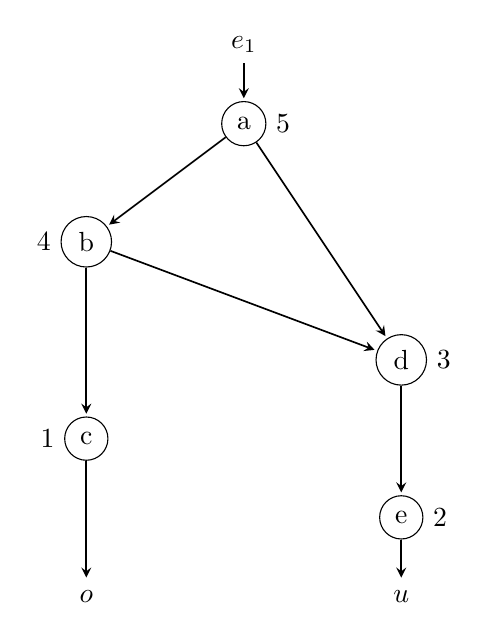
\begin{tikzpicture}
    [pre/.style={<-,shorten <=1pt,>=stealth,semithick}]
    \node (s) at (2,5) {\(e_1\)};
    \node [shape=circle,draw=black] (a) [label=right:5] at (2, 4) {a}
      edge [pre] (s);
    \node [shape=circle,draw=black] (b) [label=left:4] at (0,2.5) {b}
      edge [pre] (a);
    \node [shape=circle,draw=black] (c) [label=left:1] at (0,0) {c}
      edge [pre] (b);
    \node [shape=circle,draw=black] (d) [label=right:3] at (4,1) {d}
      edge [pre] (a)
      edge [pre] (b);
    \node [shape=circle,draw=black] (e) [label=right:2] at (4,-1) {e}
      edge [pre] (d);
    \node (o1) at (0,-2) {\(o\)} edge [pre] (c);
    \node (o2) at (4,-2) {\(u\)} edge [pre] (e);
  \end{tikzpicture}
  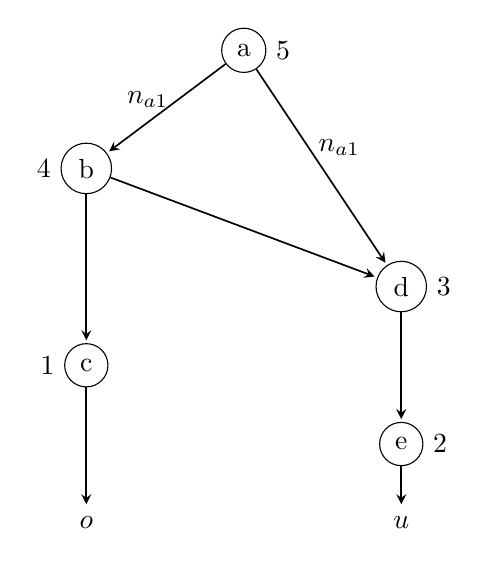
\begin{tikzpicture}
    [pre/.style={<-,shorten <=1pt,>=stealth,semithick}]
    \node [shape=circle,draw=black] (a) [label=right:5] at (2, 4) {a};
    \node [shape=circle,draw=black] (b) [label=left:4] at (0,2.5) {b}
      edge [pre] node[align=left,left,pos=0.6] {\(n_{a1}\)} (a);
    \node [shape=circle,draw=black] (c) [label=left:1] at (0,0) {c}
      edge [pre] (b);
    \node [shape=circle,draw=black] (d) [label=right:3] at (4,1) {d}
      edge [pre] node[align=right,right,pos=0.6] {\(n_{a1}\)} (a)
      edge [pre] (b);
    \node [shape=circle,draw=black] (e) [label=right:2] at (4,-1) {e}
      edge [pre] (d);
    \node (o1) at (0,-2) {\(o\)} edge [pre] (c);
    \node (o2) at (4,-2) {\(u\)} edge [pre] (e);
  \end{tikzpicture}
  \caption{Visualization of a simple asynchronous system with a reversed topological order.}
\label{fig:chap3:sec_sync:visual_dag}
\end{figure}

Figure~\ref{fig:chap3:sec_sync:visual_dag} visualizes a synchronous evaluation engine.
It shows two \glspl{dag} representations of an evaluation engine  where the nodes a to e are labeled in a reversed topological order and \(o\) and \(u\) represents the output streams with that name.
The left system is in its initial state and an input event \(e_1\) is present and can be consumed by the input node a.
When a node is chosen to compute by the scheduler, only node a is enabled, therefore it is scheduled.
The right system is the representation of the next step: node a has consumed the external event and produced an internal event \(n_{a1}\), which is propagated to all it's children: node b and d.
In the next step node b would be scheduled, because it has the lowest number of any node that can compute (actually it's the only node that can compute at all, because d has to wait for the event from b).
After b was scheduled, it would have produced the internal event \(n_{b1}\) which would then be distributed to nodes c and d.

The complete run of the synchronous engine for one input is the following, where the states are not further defined:

\begin{align*}
  \langle
    (\lambda,                             s_0),
    ((\{ n_{a1}         \}, \{n_{b1}\}),  s_1),
    ((\{ n_{b1}         \}, \{o_1\}),     s_2),\\
    ((\{ n_{a1}, n_{b1} \}, \{n_{d1}\}),  s_3),
    ((\{ n_{d1}         \}, \{u_1\}),     s_4)
  \rangle
\end{align*}

If there were more then one input event, at this point node a would be scheduled again.
It would consume the next external event and the following nodes would be scheduled in the same order as before, extending the run in an obvious way.

\subsection{Asynchronous Evaluation}
\label{sec:concepts:behaviour_without_timing:async}

An asynchronous evaluation engine is one with a fair, but not fixed schedule.

In contrast to the synchronous evaluation engine it has no fixed schedule, the only requirement is that the schedule is fair.
Therefore predecessors of enabled nodes can perform multiple computations before their children are scheduled and events are not \emph{pushed} through the \gls{dag} as fast as possible.
\todo{more later}

\section{Equivalence of Different Schedules Without Timing Functions}
\label{sec:concepts:equivalence_without_timing}

Based on the described behaviours of the approaches we now can proof the equivalence of different schedules for the same evaluation engine for a \gls{tessla} specification.

\begin{lemma}[name = Equivalence of Engines for one Input]\label{lemma:eval_equivalent_if_runs_equal}
  Two evaluation engines are equivalent for an input, if their runs are equivalent for that input.
\end{lemma}

\begin{proof}
  Since two runs are equal if they have the same last state, and all events which were produced are stored in the state, during both runs the same output events had to be generated or else their state would differ.
\end{proof}

As defined by definition~\ref{def:valid_eval_engine} any evaluation engine has to be equivalent to a synchronous one to be valid.

The equivalence is shown in two steps: first in Section~\ref{sec:concepts:equivalence_without_timing:synchronous} it is shown, that all possible synchronous engines for a specification are equivalent, so there is only one valid evaluation for a specification over a fixed input.
Afterwards in Section~\ref{sec:concepts:equivalence_without_timing:sync_async} it is shown that any asynchronous evaluation engine is equivalent to a synchronous one.


\subsection{Equivalence of Synchronous Systems}
\label{sec:concepts:equivalence_without_timing:synchronous}

When given a series of input events, two synchronous evaluation engines for a specification with different schedules will have different runs.
But both will produce all outputs that can be produced after consuming one specific input before the next input is consumed as reasoned in Section~\ref{sec:concepts:behaviour_without_timing:synchronous}.
Also both runs will obviously have the same length (both engines are the same \gls{dag}, so they have the same number of nodes), let that length be \(l\).

To proof the equivalence of both engines we can prove the equivalence of their runs.
To show the equivalence we will show that there is always another run, which is equivalent to the second one, that is closer to the first one.
If such a closer run always exist, we will show that the run with closeness \(l, 0\) to the first run, which has to be the first run itself, is also an equivalent run to the second run.

\begin{theorem}[name = Equivalence of Different Synchronous Evaluation Engines]\label{theorem:equivalence_sync_eval_engines}
  Two synchronous evaluation engines for a specification with different schedules are equivalent.
\end{theorem}
\begin{proof}

  Let \(r_1, r_2\) be the runs of the two engines for a given \gls{tessla} specification.
  Because each \gls{tessla} specification contains only a finite amount of functions and works on finite traces, the runs also have to be finite.

If the two runs aren't equal, they must have a closeness which is smaller than \((l, 0)\).
Let \([r_2]\) be the set of all runs that are equivalent to \(r_2\).
All of those runs will also have a closeness from \(r_1\) which is smaller than \((l, 0)\).
Select one run \(r_2' \in [r_2]\) which has a minimal closeness from \(r_1\).
Let \((d,k) = \delta(r_1, r_2')\).

This means that at step \(d\) the run \(r_2'\) has taken a different transition than run \(r_1\).
Let the transitions the runs have taken be \(\tau_1\) for \(r_1\) and \(\tau_2\) for \(r_2'\).
Run \(R_2'\) will take transition \(\tau_1\) at step \(d+k\) (as per the definition of the closeness).
Obviously the two transitions have to be independent of each other, else they couldn't have been taken in different order by the two runs.

If \(k > 1\) there will be a transition \(\tau_2' \neq \tau_1\) which is taken by the run \(r_2'\) at step \(d+(k-1)\).
While this transition \(\tau_2'\) must also be taken in the first run as per Lemma~\ref{lemma:enabled_till_scheduled}, it's not possible, that it was taken before \(\tau_1\), beause then the two runs wouldn't have been the same upto the point where \(\tau_1\) was taken.
Therefore \(\tau_1\) has to be independent of \(\tau_2'\), and because \(\tau_2'\) was scheduled by the second run before \(\tau_1\) both transitions are independent of each other.

As of Lemma~\ref{lemma:independent_nodes} which one of them is taken first can't change the enabledness of the node of the second transition.
Therefore there is a run \(r_2''\), which is equal to \(r_2'\), except that the transitions \(\tau_1, \tau_2'\) are scheduled the other way around.
Figure~\ref{fig:chap3:sec_sync:commutativity_scheduling} visualizes how changing the order of the two transitions can't change the global state of the engine after both were taken.
Therefore the runs \(r_2'\) and \(r_2''\) are equivalent and their closeness to \(r_1\) is \(d, k-1\), which contradicts the initial statement that \(r_1'\) was a run with a maximal closeness.
This means that there is an equivalent run to \(r_2\) which has at least the closeness \((d, 1)\).

If \(k = 1\) the transition \(\tau_2'\) from the previous case is equal to \(\tau_2\).
Based on the same reasoning there also exist a run \(r_2''\) which is equal to \(r_2'\), except that the order of \(\tau_2\) and \(\tau_1\) is changed, and which is also equivalent to \(r_2'\) and to \(r_2\).
This run has the closeness \((d, 0)\) to \(r_1\).
This obviously doesn't make sense: The first element of the closeness is the last step where both runs are equal, the second element describes how many steps afterwards the differing transition was taken.
But if it was taken right in the step after the last equal step, there is no difference at that position, so the closeness of \(r_1\) and \(r_2''\) can be at least \((d+1, x), x \in \mathbb{N}_{>0}\).
This also contradicts our initial statement that \(r_2'\) was the run with the biggest closeness to \(r_1\) which is equivalent to \(r_2\).

Combined we can now say, that there is no upper bound on the closeness of equivalent runs of \(r_2\) to \(r_1\), therefore the run with the closeness \((l, 0)\) also has to be equivalent to \(r_2\).

\end{proof}


\begin{figure}
  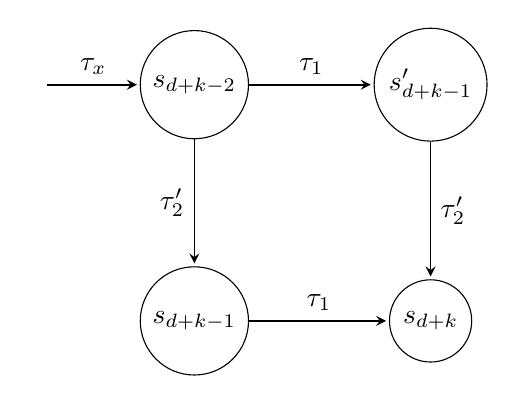
\begin{tikzpicture}
    [pre/.style={<-,shorten <=1pt,>=stealth,semithick}]
    \node (A) at (0,0) {};
    \node [shape=circle,draw=black] (B) at (2, 0) {\(s_{d+k-2}\)}
      edge [pre] node[above] {\(\tau_{x}\)} (A);
    \node [shape=circle,draw=black] (C) at (2, -3) {\(s_{d+k-1}\)}
      edge [pre] node[left] {\(\tau_{2}'\)} (B);
    \node [shape=circle,draw=black] (D) at (5, 0) {\(s_{d+k-1}'\)}
      edge [pre] node[above] {\(\tau_{1}\)} (B);
    \node [shape=circle,draw=black] (E) at (5, -3) {\(s_{d+k}\)}
      edge [pre] node[right] {\(\tau_{2}'\)} (D)
      edge [pre] node[above] {\(\tau_{1}\)} (C);
  \end{tikzpicture}
  \caption{Commutativity Diagramm of Node scheduling}
\label{fig:chap3:sec_sync:commutativity_scheduling}
\end{figure}



\subsection{Equivalence of Synchronous and Asynchronous Schedules}
\label{sec:concepts:equivalence_without_timing:sync_async}

When the nodes of \(a\) aren't scheduled in reversed topological order, the system can consume inputs before producing all outputs based on the last consumed input.
Therefore the reordering of runs has to be performed over wider parts of the run.
% Idea: each step is a commutation of two internal events in regard to the rev top order.
% => show commutativity of traces (note: only valid commutations, no two events, where one depends one the other, can be commuted, this is ensured by the scheduling of nodes that have input buffered)

\section{Behaviour with Timing functions}
\label{sec:concepts:behaviour_with_timing}
\section{Equalitys with Timing functions}
\label{sec:concepts:equivalence_with_timing}
\section{Parallel computation}
